\chapter{Analysis}

\label{Chapter4}

This section covers both the failures and success stories of the system. It is worth noting that these were uncovered after the systems were integrated, and testing was being done preparing for the competition and at the competition.

\section{Failures}

\subsection{Resource Access}
The system design did not provide a simple mechanism for acquiring resources from submarine. This lead to procedures being more complex than required, which caused an increase in procedure development time. This was because the complexity of the code lead to longer implementation and debugging time. This issue can be mitigated by implementing an interface that provides access to resources through a globally available singleton that abstracts access to all available resources. Alternatively, some abstraction offered by the control system to specific resources which the procedure would need to request.

\subsection{Navigation}
The system design missed out on the easy interface for movement that was seen in \ref{fig:DirectStateHandling}. With the predefined movement commands it was easier to add new states with different movement characteristics. This was completely overlooked on the new system design, the idea of writing procedures to complete individual tasks didn't inherently support this idea of using predefined movement commands. But seeing the results from a similar approach to navigation controls as was seen in resource access. This again caused more complex code which took longer to develop. Although it offered the highest degree of control, it was unnecessary as most of the procedures should have the movement abstracted away much like the detection system.

\subsection{Integration Testing}
The system was designed and implemented correctly. The control, navigation, and
detection systems worked individually and ran without trouble. However, during
competition there were several problems getting the submarine launched with the
three new systems with the other existing systems.

Issues arose with the launch files that are used to start all systems required
for the AUV to function. 

\begin{figure}
\centering
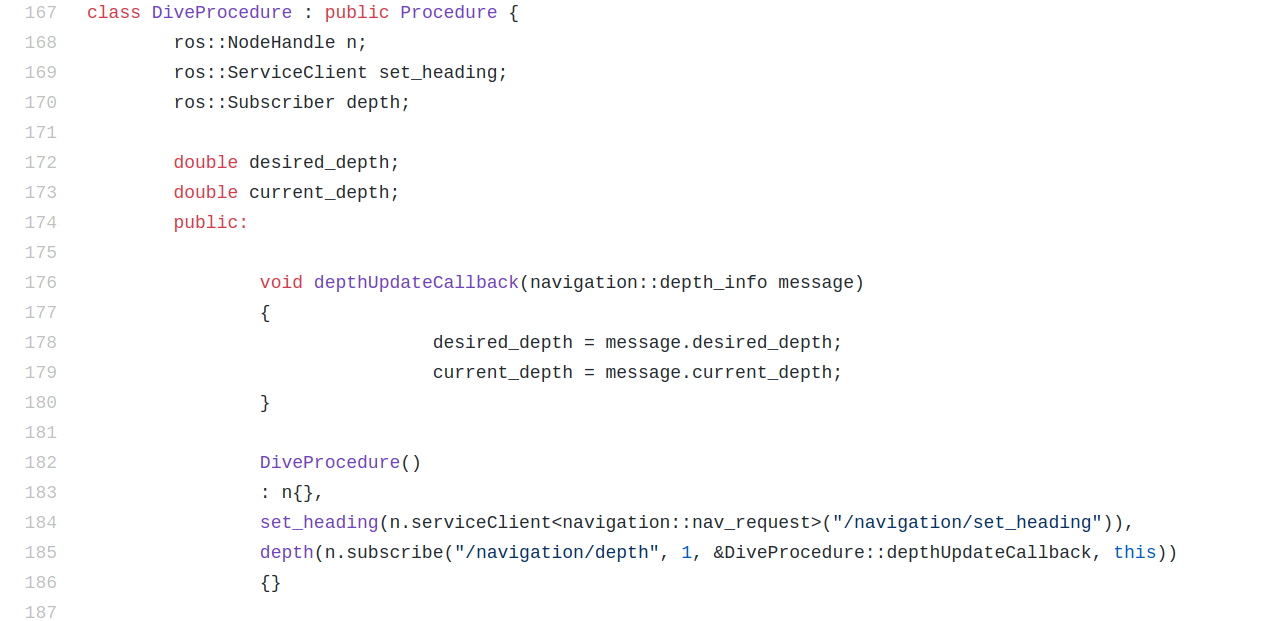
\includegraphics[width=150mm]{Figures/NewProcedureOverhead}
\decoRule
\caption[New Procedure Overhead]{Code segment shows new per-procedure overhead.}
\label{fig:NewProcedureOverhead}
\end{figure}

\section{Successes}

The dynamic loading of the state machine was a big success. It allowed the
machine to be programmed to operate in varying orders, and allows for the
control system to transition to different states alongside the next and error states.


\begin{figure}
\centering
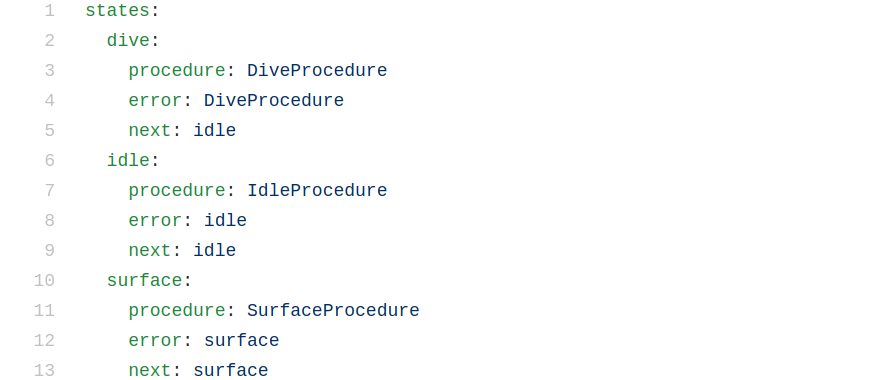
\includegraphics[width=150mm]{Figures/ExampleConfig}
\decoRule
\caption[Example Configuration File]{Shows a simple example idle configuration file. Demonstrating use of simple state organization and definition of state transitions.}
\label{fig:ExampleConfig}
\end{figure}